%%%%%%%%%%%%%%%%%%%%%%%%%%%%%%%%%
%
%       EXERCÍCIO
%
%%%%%%%%%%%%%%%%%%%%%%%%%%%%%%%%%

\definevalorquestao

\begin{exercicioBanco}[\valorquestao]
O gráfico a seguir representa a evolução da população de uma espécie animal introduzida em uma reserva ambiental ao longo de \(8\) anos.

\begin{center}
    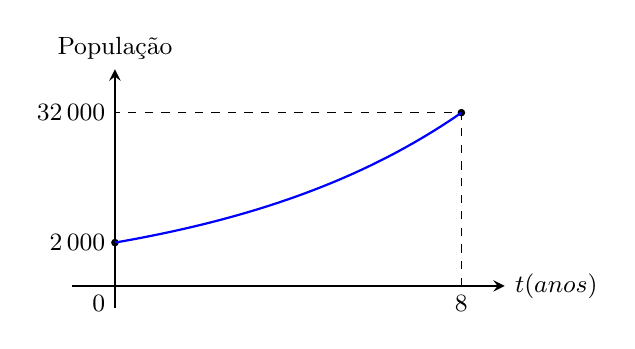
\begin{tikzpicture}[scale=0.55, >=stealth]
        % Eixos
        \draw[->, thick] (-1,0) -- (9,0) node[right] {\small $t \text{ (anos)}$};
        \draw[->, thick] (0,-0.5) -- (0,5) node[above] {\small População};
        
        % Linhas pontilhadas
        \draw[dashed] (8,0) -- (8,4) -- (0,4);
        
        % Pontos e marcações
        \fill (0,1) circle (2.5pt);
        \fill (8,4) circle (2.5pt);
        \node[left] at (0,1) {\small \(2\,000\)};
        \node[left] at (0,4) {\small \(32\,000\)};
        \node[below left] at (0,0) {\small \(0\)};
        \node[below] at (8,0) {\small \(8\)};

        % Curva exponencial f(t) = 2000 * 2^(t/2) -> f(t) = 1 * (2^(1/2))^t na escala
        \draw[domain=0:8, smooth, samples=100, thick, blue] 
            plot (\x, {2^(\x/4)});
    \end{tikzpicture}
\end{center}

Admitindo que a lei de formação que descreve essa população é dada por \(f(t) = k \cdot a^t\), os valores de \(k\) e de \(a\) são, respectivamente:

\newcommand{\alternativas}{%
    \begin{center}
        \begin{tabularx}{\textwidth}{XXX}
            (a) \(k = 2\,000\) e \(a = 16\). &
            (b) \(k = 2\,000\) e \(a = 2\). &
            (c) \(k = 32\,000\) e \(a = \sqrt[4]{2}\). \\[5pt]
            (d) \(k = 1\,000\) e \(a = 4\). &
            (e) \(k = 2\,000\) e \(a = \sqrt{2}\).
        \end{tabularx}
    \end{center}
}

\newcommand{\resposta}{E}

% Lógica condicional para exibição
\ifdefstring{\atividade}{lista}{%
    \alternativas
    \vspace{0.5em}
    
    \noindent\textbf{Resposta:} letra \textbf{\resposta}.
}{%
    \ifdefstring{\modo}{objetivo}{%
        \alternativas
    }{%
        % modo = discursiva → não mostra alternativas
    }
}
\end{exercicioBanco}

